\begin{figure}[t]
  \centering
  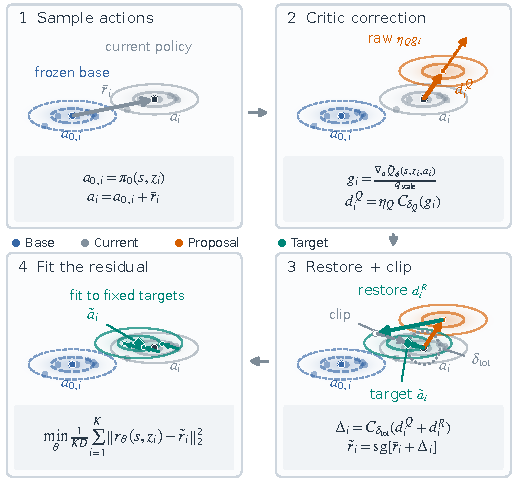
\includegraphics[width=\linewidth]{figures/method_update.pdf}
  \caption{\textbf{CAST builds fixed targets to refine robot actions.}
  At a fixed observation $s$, read clockwise: (1) sample paired base and
  current actions using the same noise $z_i$; (2) propose a clipped critic
  correction; (3) add restoration toward the base and clip the combined
  step; (4) regress the residual onto the fixed targets. In step 2, the
  dashed orange ray extends the uncapped request $\eta_Qg_i$. In step 3,
  restoration is evaluated at the current action and drawn head-to-tail
  with the critic correction; the dotted circle bounds the target step
  by $\delta_{\mathrm{tot}}$. Here
  $\bar r_i=\operatorname{sg}[r_\theta(s,z_i)]$ and
  $\tilde a_i=a_{0,i}+\tilde r_i$, where $\operatorname{sg}$ stops gradients.
  All panels share a coordinate scale; green shows the targets before actor
  fitting.}
  \label{fig:method-update}
\end{figure}
